\section{Summarized Experimental Results}\label{sec:ExperimentalResults}
This section summarizes the issues and results of the experiments, sorted by topic. In total around 17 different experimental sessions were recorded and analyzed. The earlier tests in which the experimental structure was not set yet are not included. All relevant sessions are documented on the digital appendix with their calibration patterns and example images of the image sequences. The last section describes the most successful experiment in more detail (\autoref{ssec:Session14}).

%------------------------------------------------%
% Time
%------------------------------------------------%
\paragraph{Time.}
The calibration takes a long time and the cameras are not allowed to be moved at all in the whole process. Only after all necessary calibration images are taken, it can be checked if the calibration went smoothly. In a lot of sessions the calibration had to be repeated since either the cameras were moved by accent or the calibration was not successful.

%------------------------------------------------%
% Cam set-up	
%------------------------------------------------%
\paragraph{Illumination vs. depth of field.}
The high-speed cameras need a lot of light due to their high frame rate. By keeping the cameras' aperture as open as possible the scenes get sufficient lighting but the depth of field gets very small. This results in blurred images and makes the camera calibration process very difficult. The checkerboard needs to be moved in different angles to get a good amount of calibration images, but this is hard to carry out if the depth of field is too small. More lights causes reflections on the objects and checkerboards which leads to calibration errors.

The early experimental sessions were too dark or the objects out of focus. The best results could be achieved with an aperture of 8, 4 LEDs and a distance of about 1,5 m between the cameras and the objects of interest.

\paragraph{Baseline and camera position.}
Several camera positions were tested to achieve the best results. In the first sessions (number \textit{1} to \textit{3}) the cameras were set-up on two different camera tripods with a relatively big baseline and with a rotation to each other. In \textit{session 4} the two cameras were set parallel to each other, but still with a relatively big baseline, since they were still on two separate tripods. The baseline in \textit{session 9} was decreased which resulted in more accepted image pairs in the Camera Calibrator but still did not improve the process. From \textit{session 13} onward the cameras were placed on a rig and as parallel to each other as possible. The form of the camera case and the cables still result in a baseline between 15 to 20 cm.

\paragraph{Hardware problems}
The cameras disconnected several times after which the TimeBench software and sometimes even the computer had to be restarted which was quite time-consuming. In a few sessions the cameras produced black images.

%------------------------------------------------%
% Cam calibration
%------------------------------------------------%
\paragraph{Problems with the checkerboard.}
The checkerboard detection is the most important process for the camera calibration. Next to the time-consuming factor, the checkerboard was the cause of many problems. In the early sessions (\textit{1-5} a big checkerboard in the size of a DIN A4 paper was used. The small depth of field resulted in often not fully visible or unfocused checkerboard images. The lighting was difficult as well, since reflections corrupted the images or too dark images made the checkerboard pattern not detectable. By limiting the checkerboard to fewer squares (in \textit{session 2}) and editing the images in \textit{Photoshop}\footnote{The contrast was increased and disturbing artifacts were masked.}, more image pairs were accepted by the Stereo Camera Calibrator. The stereo camera calibration bring another problem into account: if one checkerboard image is undetectable its corresponding image can not be used as well, which results in a lot less accepted image pairs.   

\textit{Session 6} used a smaller checkerboard, which was easier to handle but was too bad of a printout. The tapes with which it was glued to the paper reflected in the light and the squares were not clean enough. The capturing of the calibration images was improved by recording the calibration sequence with a lower frame rate (about 50 or 80 fps) in \textit{session 11} with which there was more time to move the pattern in different angles.

\textit{Session 12} introduced an even smaller checkerboard which was printed professionally and which had a much smoother surface. This final checkerboard had the ideal form and improved the calibration process. The square size was now 3 mm big.

\paragraph{Objects to be reconstructed}
There were different objects of interest involved in the experiments. In \textit{session 1 to 11} simple toy blocks were pushed over with a toy car. In several sessions different moving objects like a balloon (\textit{session 4}) or a toy magic wand (\textit{session 3}) were captured as well. Since the feature detection algorithms need as many different features as possible, the symmetric toy blocks were first altered with graffiti stickers (\textit{session 12}) and then completely exchanged with asymmetrical objects (\textit{session 13}).    

\paragraph{Rectification}
The biggest problem in the camera calibration process was and still is the image rectification. The rectified images are either black or do not have the correct size. Changing the cameras' position, adding more image pairs or improving the overall image quality did not change the result. The fundamental matrix computed by the Stereo Camera Calibrator seems to be incorrect. A test with normal \textit{SLR} cameras in \textit{session 13} was successful. In \textit{session 14} the rectification finally worked out fine (a discussion of this session can be found below). After this session it seemed like the error occurred when the cameras were not parallel to each other and when the baseline was too big. A later session (\textit{17}) with almost the same set-up disproved this theory. To this date it is still unclear what the causes the error. Several forum posts have similar problems but the given answers could not be applied to this situation. Solutions were: adding more image pairs and reducing the projection error by deleting outliers. All this is not relevant in these experiments since enough image pairs are accepted and the mean error is way below the recommended maximum.

\subsection{Session 14}\label{ssec:Session14}
Session 14 is the only session in which the rectification works perfectly with the footage of the high-speed cameras. The cameras were placed on a rig parallel to each other with almost no rotation with a baseline of about 20,7 cm. The cameras were triggered with an external trigger with the option \textit{falling edge}. The checkerboard's squares had the size of 3 mm and the images for calibration were captured with the help of a image sequence with 70 fps.

The actual image sequences were captured with 500 fps. Additionally several still images were taken. Although only 7 out of 19 image pairs were accepted in the Stereo Camera Calibration the rectification was successful. \autoref{fig:session1417Rectify} shows the comparison between the successful rectification of session 14 and the corrupted one of session 17 which had a very similar camera set-up.

\begin{figure}[htbp]
		\centering
		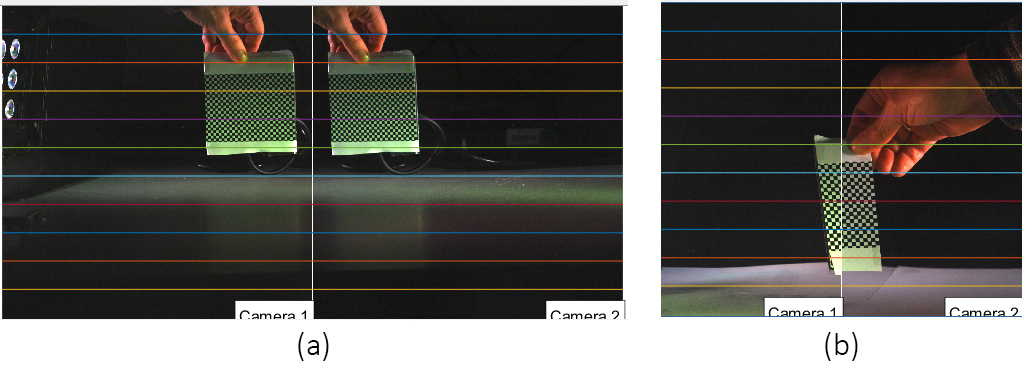
\includegraphics[width=0.8\textwidth]{figures/RectifyCompared}
		\caption[Comparison of the rectification of session 14 and 17]{Comparison of the rectification of \textbf{session 14} and \textbf{session 17}.}
		\label{fig:session1417Rectify}
\end{figure}

The extrinsic camera parameters are computed correctly (see \autoref{fig:session14Extrinsics}) and the overall mean error is with 0.11 very low.

\begin{figure}[htbp]
		\centering
		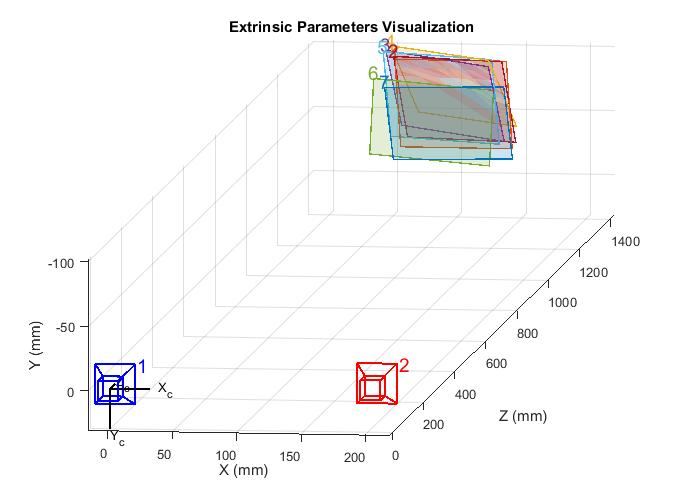
\includegraphics[width=0.8\textwidth]{figures/ExtrinsicParams}
		\caption[Extrinsic parameters of session 14]{Extrinsic parameters of session 14.}
		\label{fig:session14Extrinsics}
\end{figure}

The scenes were reconstructed smoothly. The car has the biggest problems to be detected with the algorithms. A screenshot of the reconstruction can be seen in \autoref{fig:PointCloud}.